\newcommand{\model}{%
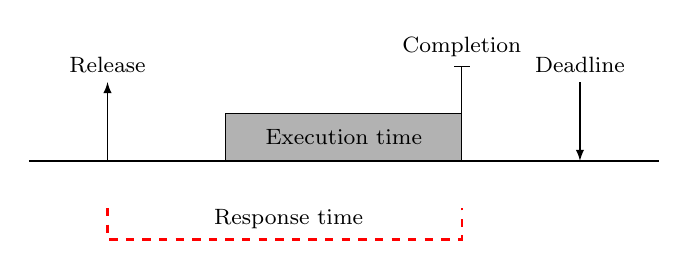
\begin{tikzpicture}[
  normal/.style={fill=black!30},
  release/.style={-latex},
  complet/.style={-|},
  every text node part/.style={align=center},
  important/.style={color=red,thick,-,dashed},
  resource/.style={ fill=black!80},
  waiting/.style={fill=white},
  busywait/.style={fill=black!10,postaction={pattern=north east lines, very thin}},
  request/.style={-o},
  unlock/.style={-*},
]
%general params
\def\th{.6} %task height
\def\blockdim{(.4,.4)}
\def\arrowdim{(0,.5)}
\def\arrowdimB{(0,.4)}

%axes
\draw[thick, black] (0,0) -- (8, 0);

%L1
\draw[release] (1, 0) -- +(0,1) node[above] {{\footnotesize Release}};
\draw[normal]  (2.5, 0) rectangle +(3, \th) node[midway] {{\footnotesize Execution time}};
\draw[complet] (5.5, 0) -- +(0, 1.2) node[above] {{\footnotesize Completion}};
\draw[release] (7, 1) node[above] {{\footnotesize Deadline}} -- (7,0);

% \draw[release] (1, 0) -- +(0,1) node[above] {{\footnotesize Release}};
% \draw[normal]  (2.5, 0) rectangle +(3, \th) node[midway] {{\footnotesize $C_i$}};
% \draw[complet] (5.5, 0) -- +(0, 1.2) node[above] {{\footnotesize Complete}};
% \draw[release] (7, 1) node[above] {{\footnotesize $P_i$ \\ \footnotesize Deadline}} -- (7,0);

\draw[important] (1,-0.6) -- (1,-1) node[above,xshift=2.3cm] {{\footnotesize {\color{black}Response time}}} --  (5.5,-1) -- (5.5,-0.6);

\end{tikzpicture}
}

\newcommand{\singleResource}{%
\begin{tikzpicture}[
  normal/.style={fill=black!30},
  release/.style={-latex},
  complet/.style={-|},
  every text node part/.style={align=center},
  important/.style={color=red,thick,-,dashed},
  resource/.style={ fill=black!80},
  waiting/.style={fill=white},
  busywait/.style={fill=black!10,postaction={pattern=north east lines, very thin}},
  request/.style={-o},
  unlock/.style={-*},
]
%general params
\def\th{.5} %task height
\def\blockdim{(.4,.4)}
\def\arrowdim{(0,.5)}
\def\arrowdimB{(0,.4)}

\def\offset{0}
%axes

%tasklines
\def\tasklinelength{(9,0)}
\draw[very thin, gray] (-.3,0)node[above,left,black]{$P$} -- +\tasklinelength;
%axes
\draw[thick, black, -] (-.2,-.5) -- (-.2, 1.3);
\draw[thick, black, ->] (-.3,-.4) -- (9, -.4) node[below] {{\footnotesize time}};
\foreach \x in {0,...,8} \draw[thin, black] (\x, -.5) -- (\x, -.3);

\path(2, -.5)node[below]{{\scriptsize $t_{1}$}};
\path(3, -.5)node[below]{{\scriptsize $t_{2}$}};

\draw[release]  (\offset + 0.0, 0) -- +(0,.8);
\draw[normal]   (\offset + 0.0, 0) rectangle +(1, \th) node[midway] {{\footnotesize $J_1$}};
\draw[request]  (\offset + 1, 0) -- +(0,.8);
\draw[resource] (\offset + 1, 0) rectangle +(1, \th)   node[color=white,midway] {{\footnotesize  $J_1$}};

\draw[release]  (\offset + 2, 0) -- +(0,.8);
\draw[normal]   (\offset + 2, 0) rectangle +(1, \th) node[midway] {{\footnotesize $J_2$}};
\draw[request]  (\offset + 3, 0) -- +(0,.8);

\draw[resource] (\offset + 3, 0) rectangle +(1, \th)   node[color=white,midway] {{\footnotesize  $J_1$}};
\draw[unlock]   (\offset + 4, 0) -- +(0,.8);

\draw[resource] (\offset + 4, 0) rectangle +(2, \th)   node[color=white,midway] {{\footnotesize  $J_2$}};
\draw[unlock]   (\offset + 6, 0) -- +(0,.8);

\draw[normal]   (\offset + 6, 0) rectangle +(1, \th) node[midway] {{\footnotesize $J_2$}};
\draw[complet]  (\offset + 7, 0) -- +(0,.8);

\draw[normal]   (\offset + 7, 0) rectangle +(1, \th) node[midway] {{\footnotesize $J_1$}};
\draw[complet]  (\offset + 8, 0) -- +(0,.8);

% \fill[busywait] (0.5, \tyOne) rectangle +(1, \th)   node[midway] {{\footnotesize $J_2$}};
% \draw[release]  (1.3, \tyOne) -- +(0,.8)            node[above]  {{\footnotesize $J_1$}};
% \draw[resource] (2.0, \tyTwo) rectangle +(1.5, \th)   node[color=white,midway] {{\footnotesize  $J_2$}};

%\draw[important] (1,-0.6) -- (1,-1) node[above,xshift=2.3cm] {{\footnotesize {\color{black}Response time}}} --  (5.5,-1) -- (5.5,-0.6);
\coordinate (legend) at (-1,2);

\draw[normal]   ($(   0,0.5) + (legend)$) node[below, xshift=0.2cm]{\scriptsize executing} rectangle +\blockdim;
\draw[resource] ($(1.75,0.5) + (legend)$) node[below, xshift=0.2cm]{\scriptsize resource} rectangle +\blockdim;
\fill[busywait] ($( 3.5,0.5) + (legend)$) node[below, xshift=0.2cm]{\scriptsize busy wait} rectangle +\blockdim;
\draw[release]  ($(5.25,0.5) + (legend)$) node[below]{\scriptsize job release}      -- +\arrowdim;
\draw[complet]  ($(   7,0.5) + (legend)$) node[below]{\scriptsize completion}   -- +\arrowdim;
\draw[request]  ($(8.75,0.5) + (legend)$) node[below]{\scriptsize request}     -- +\arrowdim;
\draw[unlock]   ($(  10.5,0.5) + (legend)$) node[below]{\scriptsize resource release}     -- +\arrowdim;

\end{tikzpicture}
}

\newcommand{\multiSuspResource}{%
\begin{tikzpicture}[
  normal/.style={fill=black!30},
  release/.style={-latex},
  complet/.style={-|},
  every text node part/.style={align=center},
  important/.style={color=red,thick,-,dashed},
  resource/.style={ fill=black!80},
  waiting/.style={fill=white},
  busywait/.style={fill=black!10,postaction={pattern=north east lines, very thin}},
  request/.style={-o},
  unlock/.style={-*},
]
%general params
\def\th{.5} %task height
\def\blockdim{(.4,.4)}
\def\arrowdim{(0,.5)}
\def\arrowdimB{(0,.4)}

\def\tyTwo{1}
\def\tyOne{0}

\def\offset{1}
%axes

%tasklines
\def\tasklinelength{(9,0)}
\draw[very thin, gray] (-.3,\tyOne)node[above,left,black]{$P_1$} -- +\tasklinelength;
\draw[very thin, gray] (-.3,\tyTwo)node[above,left,black]{$P_2$} -- +\tasklinelength;

%axes
\draw[thick, black, -] (-.2,-.5) -- (-.2, 2);
\draw[thick, black, ->] (-.3,-.4) -- (9, -.4) node[below] {{\footnotesize time}};
\foreach \x in {0,...,8} \draw[thin, black] (\x, -.5) -- (\x, -.3);

\path(3, -.5)node[below]{{\scriptsize $t_{1}$}};
\path(4, -.5)node[below]{{\scriptsize $t_{2}$}};

\draw[release]  (\offset + 0.0, \tyOne) -- +(0,.8);
\draw[normal]   (\offset + 0.0, \tyOne) rectangle +(1, \th) node[midway] {{\footnotesize $J_1$}};
\draw[request]  (\offset + 1, \tyOne) -- +(0,.8);
\draw[resource] (\offset + 1, \tyOne) rectangle +(2, \th)   node[color=white,midway] {{\footnotesize  $J_1$}};
\draw[unlock]   (\offset + 3, \tyOne) -- +(0,.8);
\draw[normal]   (\offset + 3, \tyOne) rectangle +(1, \th) node[midway] {{\footnotesize $J_1$}};
\draw[complet]  (\offset + 4, \tyOne) -- +(0,.8);

\draw[release]  (2, \tyTwo) -- +(0,.8);
\draw[normal]   (2, \tyTwo) rectangle +(1, \th) node[midway] {{\footnotesize $J_2$}};
\draw[request]  (3, \tyTwo) -- +(0,.8);

\draw[resource] (4, \tyTwo) rectangle +(2, \th)   node[color=white,midway] {{\footnotesize  $J_2$}};
\draw[unlock]   (6, \tyTwo) -- +(0,.8);
\draw[normal]   (6, \tyTwo) rectangle +(1, \th) node[midway] {{\footnotesize $J_2$}};
\draw[complet]  (7, \tyTwo) -- +(0,.8);


% \fill[busywait] (0.5, \tyOne) rectangle +(1, \th)   node[midway] {{\footnotesize $J_2$}};

\end{tikzpicture}
}

\newcommand{\multiBusyWaitResource}{%
\begin{tikzpicture}[
  normal/.style={fill=black!30},
  release/.style={-latex},
  complet/.style={-|},
  every text node part/.style={align=center},
  important/.style={color=red,thick,-,dashed},
  resource/.style={ fill=black!80},
  waiting/.style={fill=white},
  busywait/.style={fill=black!10,postaction={pattern=north east lines, very thin}},
  request/.style={-o},
  unlock/.style={-*},
]
%general params
\def\th{.5} %task height
\def\blockdim{(.4,.4)}
\def\arrowdim{(0,.5)}
\def\arrowdimB{(0,.4)}

\def\tyTwo{1}
\def\tyOne{0}

\def\offset{1}
%axes

%tasklines
\def\tasklinelength{(9,0)}
\draw[very thin, gray] (-.3,\tyOne)node[above,left,black]{$P_1$} -- +\tasklinelength;
\draw[very thin, gray] (-.3,\tyTwo)node[above,left,black]{$P_2$} -- +\tasklinelength;

%axes
\draw[thick, black, -] (-.2,-.5) -- (-.2, 2);
\draw[thick, black, ->] (-.3,-.4) -- (9, -.4) node[below] {{\footnotesize time}};
\foreach \x in {0,...,8} \draw[thin, black] (\x, -.5) -- (\x, -.3);

\path(3, -.5)node[below]{{\scriptsize $t_{1}$}};
\path(4, -.5)node[below]{{\scriptsize $t_{2}$}};

\draw[release]  (\offset + 0.0, \tyOne) -- +(0,.8);
\draw[normal]   (\offset + 0.0, \tyOne) rectangle +(1, \th) node[midway] {{\footnotesize $J_1$}};
\draw[request]  (\offset + 1, \tyOne) -- +(0,.8);
\draw[resource] (\offset + 1, \tyOne) rectangle +(2, \th)   node[color=white,midway] {{\footnotesize  $J_1$}};
\draw[unlock]   (\offset + 3, \tyOne) -- +(0,.8);
\draw[normal]   (\offset + 3, \tyOne) rectangle +(1, \th) node[midway] {{\footnotesize $J_1$}};
\draw[complet]  (\offset + 4, \tyOne) -- +(0,.8);

\draw[release]  (2, \tyTwo) -- +(0,.8);
\draw[normal]   (2, \tyTwo) rectangle +(1, \th) node[midway] {{\footnotesize $J_2$}};
\draw[request]  (3, \tyTwo) -- +(0,.8);
\fill[busywait] (3, \tyTwo) rectangle +(1, \th)   node[midway] {{\footnotesize $J_2$}};
\draw[resource] (4, \tyTwo) rectangle +(2, \th)   node[color=white,midway] {{\footnotesize  $J_2$}};
\draw[unlock]   (6, \tyTwo) -- +(0,.8);
\draw[normal]   (6, \tyTwo) rectangle +(1, \th) node[midway] {{\footnotesize $J_2$}};
\draw[complet]  (7, \tyTwo) -- +(0,.8);


\end{tikzpicture}
}